%======================================================================
\chapter{Why variational formulations matter}\label{ch:var}
%======================================================================
% Sources: "Why variational formulations matter in functional analysis"
% (v4), lecture notes C1, slides L01-L02 (constraints, Legendre-Fenchel).

\framepart{Outline}
This chapter develops a single idea: a wide class of elliptic boundary value
problems can be recast as variational problems, and this reformulation is not
a cosmetic convenience. It is the natural entry point into existence theory,
numerical methods and convex duality. The chapter starts from a discrete
structure, a chain of springs, where everything reduces to linear algebra.
It then follows one running example, the Poisson problem $-\Delta u=f$,
extended progressively to general elliptic operators, nonlinear energies,
constraints and finite elements.

\paragraph{By the end of this chapter you should be able to:}
\begin{itemize}
  \item derive the weak form of a linear elliptic PDE from its strong form,
  and conversely, using the integration-by-parts formulae of
  Appendix~\ref{app:ibp};
  \item state and apply the direct method of the calculus of variations and
  the Lax--Milgram theorem to establish existence and uniqueness;
  \item construct the dual (complementary-energy) problem with the
  Legendre--Fenchel transform, and treat constraints with Lagrange
  multipliers;
  \item recognize the structure $\mat{B}\T\mat{C}\mat{B}$ underlying springs,
  circuits, trusses and finite elements;
  \item derive a strong PDE from an energy, reconstruct an energy from a
  symmetric weak form, and recognize when no energy exists.
\end{itemize}

\paragraph{Plan of the chapter.} Section~\ref{sec:var-intro} explains why the question
matters. Section~\ref{sec:var-discrete} works out the discrete picture:
springs, the Tonti diagram, the minimum of the energy, symmetry and
reciprocity. Sections~\ref{sec:var-weak}--\ref{sec:var-elliptic} pass to the
continuum: weak and strong forms, existence by minimization, the
Lax--Milgram theorem and general elliptic operators.
Section~\ref{sec:var-dual} constructs the dual problem,
Section~\ref{sec:var-lagrange} adds constraints, Section~\ref{sec:var-fem}
discretizes by finite elements, and Section~\ref{sec:var-phys} returns to
physics with minimal surfaces. A summary, exercises with solutions
(page~\pageref{sec:var-exo}) and the references close the chapter. The technical definitions of the variational
derivatives (G\^ateaux, Fr\'echet, functional derivative) are given in
Appendix~\ref{app:derivatives}.

%======================================================================
\section{Introduction}\label{sec:var-intro}
\index{variational formulation}\index{weak form}\index{Euler--Lagrange equation}\index{Tonti diagram}%
Variational formulations translate differential or operator equations into
problems of minimizing, or finding critical points of, a functional over a
well-chosen function space. This translation unlocks the tools of functional
analysis: compactness, convexity, duality and fixed-point
arguments~\cite{Evans2010,Brezis2011,Dacorogna2008}. In practice it allows us
\begin{itemize}
  \item to construct the \emph{weak form} of a PDE, which is what finite
  elements discretize;
  \item to derive a PDE from an energy: the \emph{Euler--Lagrange equation};
  \item to recognize the dual kinematic/static structure, the \emph{Tonti
  diagram}, underlying all elliptic equations;
  \item to understand why the basic properties (symmetry, positivity,
  boundary conditions) matter, and how the continuous and discrete forms
  correspond.
\end{itemize}
Integration by parts, in the form of the Gauss--Ostrogradsky (divergence)
theorem, is used throughout; the whole family of identities is collected in
Appendix~\ref{app:ibp}. The model problem of the chapter is

\begin{gbox}{Model problem}
\index{Poisson problem}\index{energy!Dirichlet}%
\begin{equation}\label{eq:poisson}
  -\Delta u = f \ \text{in } \Omega, \qquad u = 0 \ \text{on } \partial\Omega,
  \qquad f \in L^2(\Omega),
\end{equation}
with $\Omega\subset\R^n$ a bounded Lipschitz domain. Its energy is
\begin{equation}\label{eq:poisson-energy}
  J(v) = \frac12\int_\Omega |\nabla v|^2\dd x - \int_\Omega f v\dd x,
  \qquad v\in V=H^1_0(\Omega).
\end{equation}
\end{gbox}

%======================================================================
\section{A discrete prelude: springs and the matrix \texorpdfstring{$\mat{B}\T\mat{C}\mat{B}$}{BtCB}}\label{sec:var-discrete}
Gilbert Strang's \emph{Introduction to Applied Mathematics}~\cite{Strang1986}
organizes a large range of equilibrium problems around a single diagram. It
is the discrete skeleton of every continuum problem of this book, and the
place where the main ideas can be seen with linear algebra alone.

\subsection{Positive definiteness of \texorpdfstring{$\mat{A}\T\mat{A}$}{AtA} and \texorpdfstring{$\mat{A}\T\mat{C}\mat{A}$}{AtCA}}
\begin{proposition}\label{prop:AtCA}
\index{positive definiteness!of AtCA@of $\mat{A}\T\mat{C}\mat{A}$}\index{least squares}%
Let $\mat{A}$ be an $m\times n$ matrix ($n\le m$) with independent columns.
Then $\mat{A}\T\mat{A}$ is symmetric positive definite. More generally, if
$\mat{C}$ is symmetric positive definite, so is $\mat{A}\T\mat{C}\mat{A}$.
\end{proposition}
\begin{proof}
For any $\vx\in\R^n$, $\vx\T\mat{A}\T\mat{A}\vx=|\mat{A}\vx|^2\ge0$, and
$|\mat{A}\vx|=0$ implies $\mat{A}\vx=\vzero$, hence $\vx=\vzero$ since the
columns of $\mat{A}$ are independent. Symmetry is immediate. In the general
case, with $|\vect{y}|_{\mat{C}}^2=\vect{y}\T\mat{C}\vect{y}$,
$\vx\T\mat{A}\T\mat{C}\mat{A}\vx=|\mat{A}\vx|_{\mat{C}}^2$, which is a norm
because $\mat{C}>0$; the same argument applies.
\end{proof}
For $\mat{A}\vx=\vb$, the normal equations $\mat{A}\T\mat{A}\vx=\mat{A}\T\vb$
are the equations of least squares; $\mat{A}\T\mat{A}$ can be analysed with
the singular value decomposition of $\mat{A}$. Note that $\mat{A}$ need not
be invertible, nor even square: only the independence of its columns is
required.

\subsection{A chain of springs}\label{ssec:springs}
\index{spring chain}\index{compatibility}\index{equilibrium!discrete}\index{constitutive law!Hooke (springs)}%
Consider four springs connecting three masses between two fixed walls.
\begin{center}
\begin{tikzpicture}[scale=1]
  \draw[thick] (0,-0.5) -- (0,0.5);
  \foreach \y in {-0.5,-0.3,-0.1,0.1,0.3,0.5} \draw (0,\y) -- (-0.18,\y-0.18);
  \draw[thick] (9,-0.5) -- (9,0.5);
  \foreach \y in {-0.5,-0.3,-0.1,0.1,0.3,0.5} \draw (9,\y) -- (9.18,\y-0.18);
  \draw[spring] (0,0) -- (2,0);      \node[above] at (1,0.28) {\small $e_1,\,\sigma_1$};
  \draw[spring] (2.5,0) -- (4.25,0); \node[above] at (3.375,0.28) {\small $e_2,\,\sigma_2$};
  \draw[spring] (4.75,0) -- (6.5,0); \node[above] at (5.625,0.28) {\small $e_3,\,\sigma_3$};
  \draw[spring] (7,0) -- (9,0);      \node[above] at (8,0.28) {\small $e_4,\,\sigma_4$};
  \foreach \i/\xpos in {1/2.25, 2/4.5, 3/6.75} {
    \draw[thick,fill=white] (\xpos,0) circle (0.25);
    \node at (\xpos,0) {$m_{\i}$};
    \draw[arr] (\xpos,-0.35) -- (\xpos,-0.85);
    \node[below] at (\xpos,-0.85) {$u_{\i},\,f_{\i}$};
  }
\end{tikzpicture}
\end{center}
Let $\vu=(u_1,u_2,u_3)$ be the nodal displacements, $\ve=(e_1,\dots,e_4)$ the
spring elongations, $\vect{\sigma}=(\sigma_1,\dots,\sigma_4)$ the spring
forces and $\vf$ the external nodal forces. The three groups of equations are:
\begin{itemize}
\item \emph{kinematics} (compatibility), $\ve=\mat{B}\vu$:
\[
  \begin{bmatrix} e_1\\ e_2\\ e_3\\ e_4 \end{bmatrix}
  =\begin{bmatrix} 1 & & \\ -1 & 1 & \\ & -1 & 1 \\ & & -1 \end{bmatrix}
  \begin{bmatrix} u_1 \\ u_2 \\ u_3 \end{bmatrix};
\]
\item \emph{constitutive law} (Hooke), $\vect{\sigma}=\mat{C}\ve$, with
$\mat{C}=\diag(c_1,c_2,c_3,c_4)$ the spring stiffnesses;
\item \emph{equilibrium} of each mass, $\vf=\mat{B}\T\vect{\sigma}$:
\[
  \begin{bmatrix} f_1 \\ f_2 \\ f_3 \end{bmatrix}
  =\begin{bmatrix} 1 & -1 & & \\ & 1 & -1 & \\ & & 1 & -1 \end{bmatrix}
  \begin{bmatrix} \sigma_1\\ \sigma_2\\ \sigma_3\\ \sigma_4 \end{bmatrix}.
\]
\end{itemize}
Combining, $\vf=\mat{B}\T\vect{\sigma}=\mat{B}\T\mat{C}\mat{B}\,\vu=\mat{K}\vu$.

\paragraph{$\mat{B}\T$ and $\mat{B}$ are transposes, and not by accident.} The
\index{virtual work!discrete}\index{transpose and adjoint}%
internal work done stretching the springs equals the external work done at
the nodes,
\[
  \vect{\sigma}\T\ve=\vect{\sigma}\T\mat{B}\vu=\vf\T\vu ,
\]
and this identity holds for \emph{every} displacement $\vu$ only if the
equilibrium operator is exactly $\mat{B}\T$. This is the discrete principle of
virtual work; its continuum version is the pair
$\nabla\leftrightarrow-\dive$ of Appendix~\ref{app:ibp}.

With unit stiffnesses, $\mat{K}=\mat{B}\T\mat{B}=\operatorname{tridiag}(-1,2,-1)$:
\[
  \mat{K}=\begin{pmatrix} 2 & -1 & 0 \\ -1 & 2 & -1 \\ 0 & -1 & 2 \end{pmatrix}.
\]
For a uniform unit load $\vf=(1,1,1)\T$, symmetry ($u_1=u_3$) and
back-substitution give $\vu=(\tfrac32,\,2,\,\tfrac32)\T$, a discrete
parabola. As the number of masses grows it converges to the solution
$u(x)=\tfrac12x(1-x)$ of $-u''=1$, $u(0)=u(1)=0$; the same matrix reappears as
the finite element stiffness matrix in Section~\ref{sec:var-fem}.

\subsection{Duality: the Tonti diagram}
\index{Tonti diagram!discrete}\index{stiffness matrix}%
\begin{figure}[h]
\centering
\begin{tikzpicture}[node distance=1.4cm and 3.6cm]
  \node[smallbox] (x) {$\vu$ \\ \footnotesize displacement};
  \node[smallbox, right=3.6cm of x] (f) {$\vf$ \\ \footnotesize force};
  \node[smallbox, below=1.4cm of x] (e) {$\ve=\mat{B}\vu$ \\ \footnotesize elongation};
  \node[smallbox, below=1.4cm of f] (s) {$\vect{\sigma}=\mat{C}\ve$ \\ \footnotesize spring force};
  \draw[arr] (x) -- (e) node[midway,left]{$\mat{B}$};
  \draw[arr] (e) -- (s) node[midway,below]{$\mat{C}$};
  \draw[arr] (s) -- (f) node[midway,right]{$\mat{B}\T$};
  \node[left=0.3cm of e,font=\scriptsize\sffamily,align=right] {kinematic};
  \node[right=0.3cm of s,font=\scriptsize\sffamily,align=left] {static};
\end{tikzpicture}
\caption{Tonti diagram of the spring chain. Top row: primary fields; bottom
row: derived fields, kinematic on the left, static on the right, joined by
the material law $\mat{C}$.}
\label{fig:tonti-discrete}
\end{figure}
Figure~\ref{fig:tonti-discrete} shows the structure. By
Proposition~\ref{prop:AtCA}, $\mat{K}=\mat{B}\T\mat{C}\mat{B}$ is symmetric
and positive definite as soon as $\mat{C}>0$ and $\mat{B}$ has independent
columns, i.e.\ as soon as the structure has no rigid-body motion. The
associated energy is
\begin{equation}\label{eq:W-discrete}
  W(\vu)=\tfrac12\vu\T\mat{B}\T\mat{C}\mat{B}\,\vu-\vu\T\vf
        =\tfrac12\ve\T\vect{\sigma}-\vu\T\vf ,
\end{equation}
the internal potential energy minus the work of the external forces.

\subsection{The minimum of the energy}
\begin{theorem}\label{thm:min-discrete}
\index{energy!minimum (discrete)}\index{minimum principle!discrete}%
Let $\mat{K}$ be symmetric positive definite and
$W(\vu)=\tfrac12\vu\T\mat{K}\vu-\vu\T\vf$. Then $W$ is minimal exactly at the
solution of $\mat{K}\vu=\vf$, and $W_{\min}=-\tfrac12\vf\T\mat{K}^{-1}\vf$.
\end{theorem}
\begin{proof}
Let $\mat{K}\vu=\vf$ and let $\vv$ be arbitrary. Using $\mat{K}\vu=\vf$ to
cancel the cross terms,
\[
  W(\vv)-W(\vu)=\tfrac12(\vv-\vu)\T\mat{K}(\vv-\vu)\ge0 ,
\]
with equality only for $\vv=\vu$. Substituting $\vu=\mat{K}^{-1}\vf$ gives
$W_{\min}=\tfrac12\vf\T\mat{K}^{-1}\vf-\vf\T\mat{K}^{-1}\vf$.
\end{proof}

\begin{figure}[h]
\centering
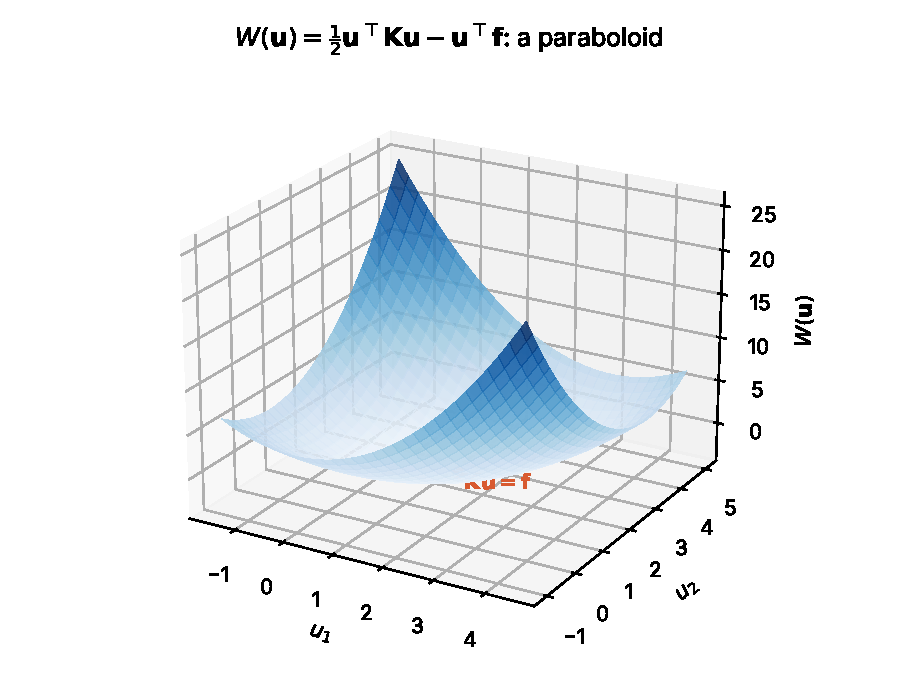
\includegraphics[width=0.6\textwidth]{figures/ch1/paraboloid.pdf}
\caption{The energy $W$ is a paraboloid: spring chain with unit stiffnesses,
$\vf=(1,1,1)\T$, sliced at the optimal $u_3$. The marked point solves
$\mat{K}\vu=\vf$, and $W_{\min}=-2.5=-\tfrac12\vf\T\mat{K}^{-1}\vf$.}
\label{fig:paraboloid}
\end{figure}

The positive definiteness of $\mat{K}$ can be quantified. Expanding $\vu$ in
\index{Rayleigh quotient}\index{coercivity!discrete}\index{boundedness!discrete}%
the orthonormal eigenbasis of $\mat{K}$ gives
\begin{equation}\label{eq:rayleigh}
  \lambda_{\min}\,|\vu|^2\le\vu\T\mat{K}\vu\le\lambda_{\max}\,|\vu|^2 .
\end{equation}
The lower bound is \emph{coercivity}, the upper bound \emph{boundedness}:
these are exactly the two hypotheses of the Lax--Milgram theorem of
Section~\ref{sec:var-lm}, here verified on a matrix
(Exercise~\ref{exo:lm-constants}).

\subsection{Symmetry, energy and path independence}\label{ssec:symmetry}
\index{symmetry!and existence of an energy}\index{path independence}%
Positive definiteness makes $W$ a genuine energy, bounded below and strictly
convex. Symmetry is what makes it exist at all. For a linear system
$\vF=\mat{K}\vu$, the work along a loading path from state $A$ to state $B$ is
\[
  \int_A^B\vF\cdot\dot\vu\dd t=\int_A^B\dot\vu\T\mat{K}\vu\dd t
  =\tfrac12\bigl[\vu\T\mat{K}\vu\bigr]_A^B
\]
\emph{if and only if $\mat{K}$ is symmetric}. Otherwise the work depends on
the path and not only on the end points, and no state function exists. The
same holds for bilinear forms: a symmetric form $a(u,v)$ has the energy
$J(u)=\tfrac12a(u,u)-L(u)$, a non-symmetric one generally has none
(Exercises~\ref{exo:guess-energy} and~\ref{exo:no-energy}).

\subsection{Reciprocity: the Maxwell--Betti theorem}\label{ssec:reciprocity}
\index{reciprocity!Maxwell--Betti}\index{Maxwell--Betti theorem}\index{Faraday experiment}%
\begin{figure}[h]
\centering
\begin{tikzpicture}[scale=1]
  \draw[thick] (0,0) -- (0,1);
  \foreach \y in {0,0.2,0.4,0.6,0.8,1} \draw (0,\y) -- (-0.18,\y-0.18);
  \draw[thick] (0,0.5) -- (4.2,0.5);
  \draw[arr,color=orange!80!black] (1.2,0.5) -- (1.2,1.1);
  \node[above,font=\small] at (1.2,1.15) {$F^{(1)}$};
  \node[below,font=\small] at (1.2,0.35) {$P$};
  \draw[arr,color=cu] (3.2,0.5) -- (3.2,0.9);
  \node[above,font=\small] at (3.2,0.95) {$u^{(1)}_Q$};
  \node[below,font=\small] at (3.2,0.35) {$Q$};
  \node[font=\sffamily\small] at (2.1,-0.35) {load case 1};
  \begin{scope}[xshift=6cm]
  \draw[thick] (0,0) -- (0,1);
  \foreach \y in {0,0.2,0.4,0.6,0.8,1} \draw (0,\y) -- (-0.18,\y-0.18);
  \draw[thick] (0,0.5) -- (4.2,0.5);
  \draw[arr,color=cu] (1.2,0.5) -- (1.2,0.9);
  \node[above,font=\small] at (1.2,0.95) {$u^{(2)}_P$};
  \node[below,font=\small] at (1.2,0.35) {$P$};
  \draw[arr,color=orange!80!black] (3.2,0.5) -- (3.2,1.1);
  \node[above,font=\small] at (3.2,1.15) {$F^{(2)}$};
  \node[below,font=\small] at (3.2,0.35) {$Q$};
  \node[font=\sffamily\small] at (2.1,-0.35) {load case 2};
  \end{scope}
\end{tikzpicture}
\caption{Reciprocity. Loading at $P$ and measuring at $Q$ gives the same
cross-work as loading at $Q$ and measuring at $P$:
$F^{(1)}u^{(2)}_P=F^{(2)}u^{(1)}_Q$.}
\label{fig:reciprocity}
\end{figure}
Loading a structure at $P$ and measuring the displacement at $Q$ gives the
same cross-work as loading at $Q$ and measuring at $P$
(Figure~\ref{fig:reciprocity}). This is the reciprocity principle, shown in
class as the ``Faraday experiment''.\footnote{In the literature the result is
credited to Clebsch ($\sim$1862), Maxwell (1864), Betti (1872) and Rayleigh
(1873).}\draftnote{Faraday attribution: keep as the name of the classroom demo?}

\begin{proposition}\label{prop:reciprocity}
\index{reciprocity!and symmetry}\index{flexibility matrix}%
Let $\vF=\mat{K}\vu$ with $\mat{K}$ invertible. The reciprocity identity
\[
  \vF^{(1)}\cdot\vu^{(2)}=\vF^{(2)}\cdot\vu^{(1)}
\]
holds for every pair of load cases if and only if $\mat{K}\T=\mat{K}$.
\end{proposition}
\begin{proof}
$\vF^{(1)}\cdot\vu^{(2)}=(\mat{K}\vu^{(1)})\T\vu^{(2)}=\vu^{(1)\top}\mat{K}\T\vu^{(2)}$
and $\vF^{(2)}\cdot\vu^{(1)}=\vu^{(1)\top}\mat{K}\vu^{(2)}$. They agree for all
$\vu^{(1)},\vu^{(2)}$ if and only if $\mat{K}\T=\mat{K}$. For unit loads at $P$
and $Q$, the displacements are columns of the flexibility matrix
$\mat{S}=\mat{K}^{-1}$, and reciprocity reads $S_{QP}=S_{PQ}$.
\end{proof}
In the continuum, reciprocity is Green's second identity
(Appendix~\ref{app:ibp}). When the body contains an unknown defect,
reciprocity between the true field and a known ``adjoint'' field is
\emph{broken}, and the gap measures the defect: this is the idea of
Chapter~\ref{ch:rg}.

\subsection{Circuits and trusses: the same linear algebra}
\paragraph{A resistor network.} Replace masses by nodes, displacements $\vu$ by
\index{resistor network}%
potentials and springs by resistors. Ohm's law $\sigma_i=c_ie_i$ is the
constitutive law, $\mat{C}=\diag(\text{conductances})$, and Kirchhoff's current
law at the nodes is exactly $\mat{B}\T\vect{\sigma}=\vf$ (injected currents).
With unit conductances the assembled matrix is the same $\mat{K}$: a resistor
ladder and a spring chain obey identical linear algebra. It is the discrete
analogue of $-\dive(\tA(\vx)\nabla u)=f$ (Section~\ref{sec:var-elliptic}).

\paragraph{A small truss.} Let $\mat{B}$ map joint displacements to bar
\index{truss}\index{energy!complementary (discrete)}%
elongations in a planar truss, $\mat{C}=\diag(E_iA_i/L_i)$ collect the bar
stiffnesses, and $\mat{B}\T\vect{\sigma}=\vf$ express the equilibrium of the
joints. Minimizing $W(\vu)$ is the discrete \emph{potential energy principle}.
Its dual, maximizing $-\tfrac12\vect{\sigma}\T\mat{C}^{-1}\vect{\sigma}$ over bar
tensions satisfying $\mat{B}\T\vect{\sigma}=\vf$, is the discrete
\emph{complementary energy principle}: the finite-dimensional counterpart of
the primal/dual pair of Section~\ref{sec:var-dual}, with $\mat{B}\T$ playing
the role of $-\dive$ and $\mat{C}^{-1}$ that of the conjugate energy.

%======================================================================
\section{Weak and strong forms: the right function space}\label{sec:var-weak}
\index{weak form}\index{strong form}\index{Sobolev space}\index{integration by parts!weak form}%
Integration by parts lowers the number of derivatives required, moving the
natural setting from $H^2$ down to $H^1$. This is why Sobolev spaces and
elliptic PDE theory are so intertwined~\cite{AdamsFournier2003,Evans2010}.
\begin{center}
\begin{tikzpicture}[node distance=1.6cm]
  \node[smallbox] (s) {Strong form \\ $-\Delta u = f,\ u \in H^2(\Omega)$};
  \node[smallbox, right=of s] (w) {Weak form \\
    $\int_\Omega \nabla u \cdot \nabla v = \int_\Omega f v,\ u,v \in H^1_0(\Omega)$};
  \draw[arr] (s) -- node[above, font=\small]{integrate} node[below,font=\small]{by parts} (w);
\end{tikzpicture}
\end{center}
Multiply $-\Delta u=f$ by a test function $v\in C_c^\infty(\Omega)$ and
integrate by parts (Green's first identity, Theorem~\ref{thm:green1}):
\[
  -\int_\Omega (\Delta u)\, v\dd x=\int_\Omega \nabla u \cdot \nabla v\dd x
  = \int_\Omega f v\dd x .
\]
The boundary term vanishes since $v=0$ near $\partial\Omega$. The left-hand
side only requires $u,v\in H^1$ (one derivative in $L^2$), so the identity
extends by density to all $v\in H^1_0(\Omega)$; there is no longer any need
for $u\in H^2$.

The weak form is also the first variation of the energy~\eqref{eq:poisson-energy}:
$\frac{\dd}{\dd t}J(u+tv)\big|_{t=0}=\int_\Omega\nabla u\cdot\nabla v-\int_\Omega fv$.
The three settings
\begin{center}
\begin{tabular}{lll}
\toprule
\sffamily energy & \sffamily weak form (virtual work) & \sffamily strong form (Euler--Lagrange)\\
\midrule
$\displaystyle u=\argmin_{v\in V}J(v)$ & $\delta J(u)[v]=0\ \ \forall v\in V$ & $-\Delta u=f$ in $\Omega$\\
\bottomrule
\end{tabular}
\end{center}
are equivalent for smooth solutions; their precise definitions are given in
Appendix~\ref{app:derivatives}.

%======================================================================
\section{Existence by minimization: the direct method}\label{sec:var-direct}
\index{direct method}\index{lower semicontinuity}\index{minimizing sequence}\index{Poincar\'e inequality}\index{coercivity!of an energy}%
Recasting a PDE as a minimization problem turns existence into the question
of whether a functional attains its infimum. Weak compactness and lower
semicontinuity answer it without constructing the solution~\cite{Dacorogna2008}.
\begin{center}
\begin{tikzpicture}[node distance=0.55cm]
  \node[box] (a) {Minimize $J(u)$ over $V$};
  \node[box, below=of a] (b) {Take a minimizing sequence $(u_n)$};
  \node[box, below=of b] (c) {Bounded $\Rightarrow$ weakly compact in $V$ (reflexive)};
  \node[box, below=of c] (d) {$J$ weakly lower semicontinuous};
  \node[box, goal, below=of d] (e) {Minimizer $u^\ast$ attained};
  \draw[arr] (a) -- (b); \draw[arr] (b) -- (c); \draw[arr] (c) -- (d); \draw[arr] (d) -- (e);
\end{tikzpicture}
\end{center}
For the energy~\eqref{eq:poisson-energy} on $V=H^1_0(\Omega)$:
\begin{itemize}
  \item \emph{coercivity:} by the Poincar\'e inequality
  $\norm{v}_{L^2}\le C_P\norm{\nabla v}_{L^2}$,
  \[
    J(v)\ge\tfrac12\norm{\nabla v}_{L^2}^2-C_P\norm{f}_{L^2}\norm{\nabla v}_{L^2}\to\infty
    \quad\text{as }\norm{v}_{H^1_0}\to\infty;
  \]
  in particular $J$ is bounded below;
  \item a minimizing sequence $(u_n)$ is therefore bounded in $H^1_0$, and a
  subsequence converges weakly to some $u$ (reflexivity);
  \item $J$ is convex and continuous, hence weakly lower semicontinuous:
  $J(u)\le\liminf J(u_n)=\inf J$.
\end{itemize}
So $u$ is a minimizer, and its first variation gives $-\Delta u=f$ in the weak
sense.

%======================================================================
\section{The Lax--Milgram theorem}\label{sec:var-lm}
\index{Lax--Milgram theorem}\index{coercivity!of a bilinear form}\index{boundedness!of a bilinear form}%
Two functional-analytic hypotheses on a bilinear form, boundedness and
coercivity, give existence \emph{and} uniqueness, independently of the
specific PDE~\cite{LaxMilgram1954}.

\begin{gbox}{Lax--Milgram theorem}
Let $V$ be a Hilbert space, $a:V\times V\to\R$ bilinear and $L\in V^\ast$.
If $a$ is \emph{bounded}, $|a(u,v)|\le M\norm{u}\norm{v}$, and \emph{coercive},
$a(u,u)\ge\alpha\norm{u}^2$ with $\alpha>0$, then there is a unique $u\in V$
such that
\[
  a(u,v)=L(v)\qquad\forall v\in V,
\]
and $\norm{u}\le\norm{L}_{V^\ast}/\alpha$. The form $a$ need not be symmetric.
\end{gbox}

For the model problem, $a(u,v)=\int_\Omega\nabla u\cdot\nabla v$ and
$L(v)=\int_\Omega fv$ on $H^1_0(\Omega)$:
\begin{itemize}
  \item \emph{bounded:} $|a(u,v)|\le\norm{\nabla u}_{L^2}\norm{\nabla v}_{L^2}$
  (Cauchy--Schwarz);
  \item \emph{coercive:} $a(u,u)=\norm{\nabla u}_{L^2}^2\ge\alpha\norm{u}_{H^1_0}^2$
  (Poincar\'e);
  \item $L$ is bounded: $|L(v)|\le\norm{f}_{L^2}\norm{v}_{L^2}\le C_P\norm{f}_{L^2}\norm{v}_{H^1_0}$.
\end{itemize}
Lax--Milgram gives existence and uniqueness directly, without mentioning
minimization. The discrete bounds~\eqref{eq:rayleigh} are the same two
hypotheses for a matrix.

\subsection*{What goes wrong without coercivity}
Boundedness alone is not enough. Two examples, one linear and one nonlinear,
show what breaks.

\paragraph{(a) A linear resonance.} On $H^1_0(0,1)$ take
\index{resonance}\index{Wirtinger inequality}\index{Fredholm alternative}%
\[
  a(u,v)=\int_0^1u'v'\dd x-\pi^2\int_0^1uv\dd x,
\]
corresponding to $-u''-\pi^2u=f$, $u(0)=u(1)=0$. The form is bounded,
$|a(u,v)|\le(1+\pi^2)\norm{u}_{H^1_0}\norm{v}_{H^1_0}$, but not coercive: the
sharp Poincar\'e (Wirtinger) inequality $\int_0^1(u')^2\ge\pi^2\int_0^1u^2$ is
an equality at $u=\sin\pi x$, so $a(\sin\pi x,\sin\pi x)=0$. This is not an
artefact of the proof: $\pi^2$ is the first Dirichlet eigenvalue of
$-\dd^2/\dd x^2$ on $(0,1)$, the problem is at resonance, and the Fredholm
alternative (Section~\ref{sec:var-elliptic}) takes over. Solvability requires
$f\perp\sin\pi x$ in $L^2$. For $f=1$, $\int_0^1\sin\pi x\dd x=2/\pi\neq0$:
\textbf{no solution}. For $f=\sin2\pi x$ the condition holds, and
$u_c=\sin(2\pi x)/(3\pi^2)+c\sin\pi x$ solves the problem for every
$c\in\R$: \textbf{infinitely many solutions} (Figure~\ref{fig:resonance}).

\begin{figure}[h]
\centering
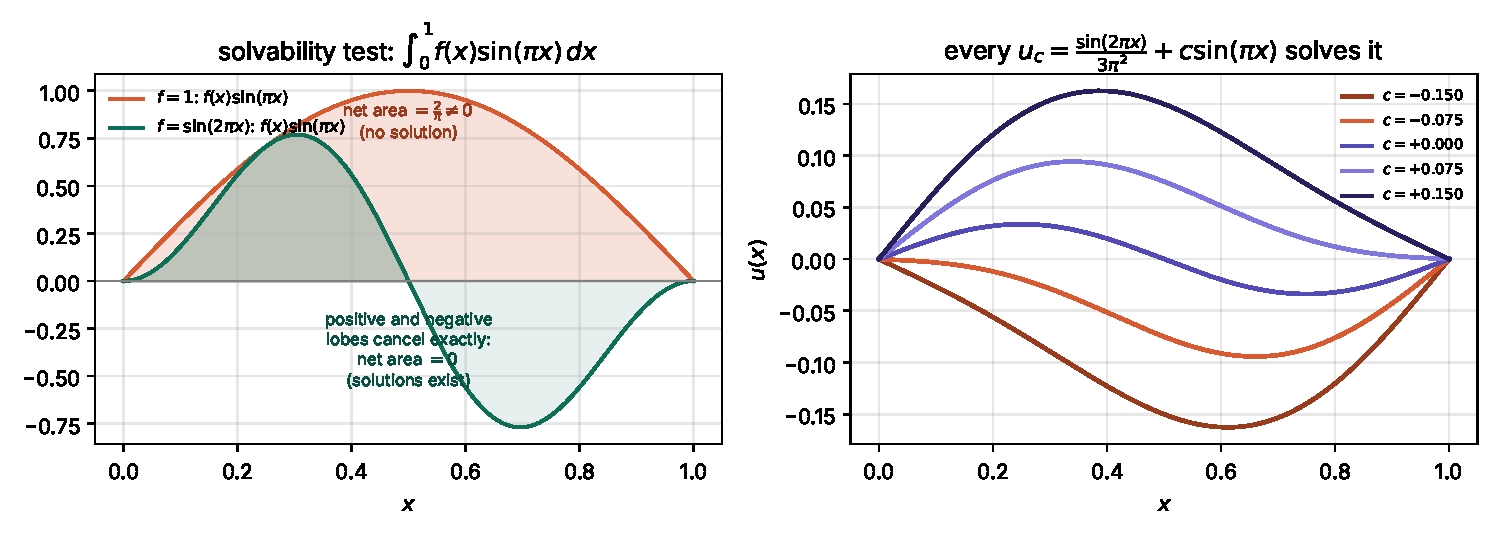
\includegraphics[width=\textwidth]{figures/ch1/resonance_example.pdf}
\caption{Resonance. Left: the solvability test $\int_0^1 f\sin\pi x\dd x$.
For $f=1$ the product stays positive and the integral is $2/\pi$: no
solution. For $f=\sin2\pi x$ the lobes cancel: solutions exist. Right: the
one-parameter family $u_c$ of solutions.}
\label{fig:resonance}
\end{figure}

\paragraph{(b) A nonlinear double well.} Lax--Milgram is a linear theorem, but
\index{double well}\index{Allen--Cahn equation}\index{second variation}\index{stability!of a critical point}%
the coercivity intuition reappears in the second variation. On $(0,1)$ take
\[
  E[u]=\int_0^1\Bigl(\frac{\varepsilon^2}{2}(u')^2+W(u)\Bigr)\dd x,
  \qquad W(u)=\tfrac14(u^2-1)^2,
\]
whose Euler--Lagrange equation is the stationary Allen--Cahn equation
$-\varepsilon^2u''+u^3-u=0$~\cite{AllenCahn1979}. Existence of a minimizer
still holds by the direct method (Rellich--Kondrachov compactness handles the
non-convex zeroth-order term), but uniqueness fails twice: by the symmetry
$u\mapsto-u$, $u\equiv1$ and $u\equiv-1$ are both global minimizers; and
$u\equiv0$ is a critical point whose second variation
\[
  \delta^2E(0)[v,v]=\varepsilon^2\int_0^1(v')^2\dd x-\int_0^1v^2\dd x
\]
is \emph{negative} for every nonzero constant $v$: $u\equiv0$ is unstable
(Figure~\ref{fig:doublewell}). Stability through the second variation is the
subject of the last part of the course.

\begin{figure}[h]
\centering
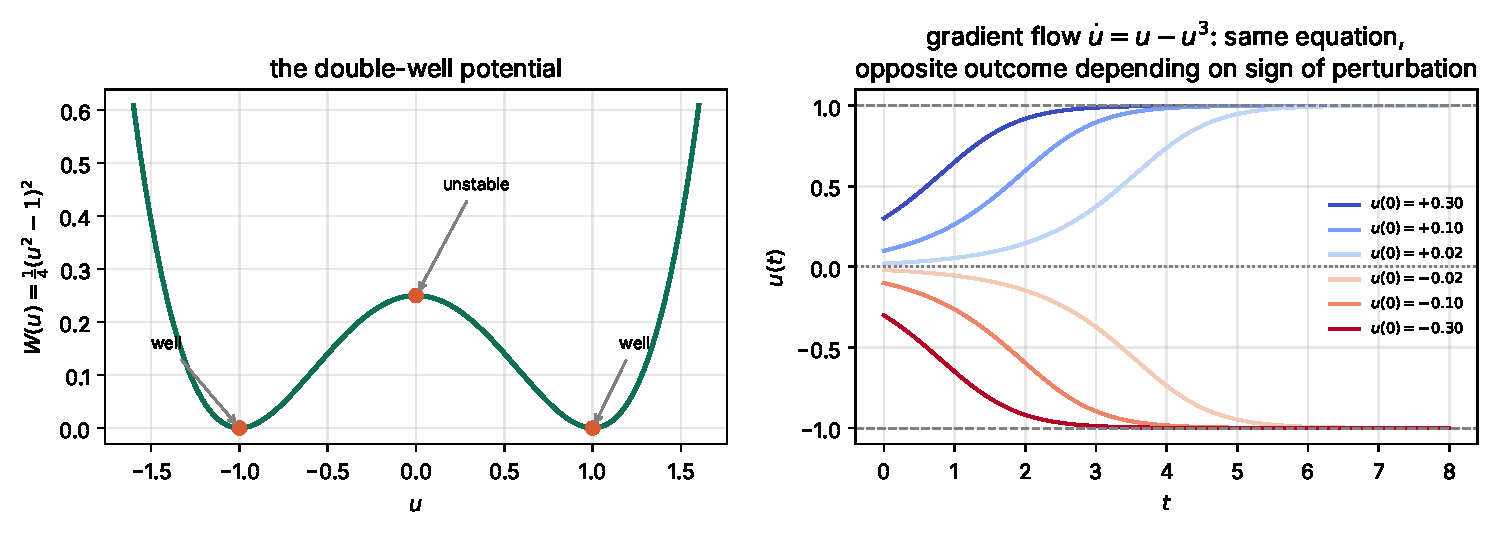
\includegraphics[width=\textwidth]{figures/ch1/doublewell_bistability.pdf}
\caption{Left: the double-well potential, minima at $u=\pm1$, unstable maximum
at $u=0$. Right: the gradient flow $\dot u=u-u^3$ from initial conditions near
$0$; a $\pm0.02$ perturbation decides whether the system ends at $+1$ or $-1$.}
\label{fig:doublewell}
\end{figure}

%======================================================================
\section{General elliptic operators}\label{sec:var-elliptic}
\index{elliptic operator!general}\index{uniform ellipticity}\index{G\aa rding inequality@G{\aa}rding inequality}%
The Poisson problem uses the simplest elliptic operator. The Lax--Milgram
framework is built for the general second-order case, where the minimization
approach does not always apply~\cite{GilbargTrudinger2001,Evans2010}.

\paragraph{The operator.} Consider
\begin{equation}\label{eq:general-elliptic}
  -\dive(\tA(\vx)\nabla u)+\vb(\vx)\cdot\nabla u+c(\vx)u=f
  \ \text{in } \Omega,\qquad u=0 \ \text{on } \partial\Omega,
\end{equation}
with $\tA(\vx)$ a second-order tensor field (conductivity, diffusivity),
$\vb$ a drift (convection) field and $c$ a reaction coefficient. The operator
is \emph{uniformly elliptic} if
$\vxi\cdot\tA(\vx)\vxi\ge\alpha|\vxi|^2$ for all $\vxi\in\R^n$, $\vx\in\Omega$,
some $\alpha>0$.

\paragraph{The bilinear form.} Integrating by parts with
Theorem~\ref{thm:ibp-matrix},
\[
  a(u,v)=\int_\Omega\tA\nabla u\cdot\nabla v\dd x
  +\int_\Omega(\vb\cdot\nabla u)\,v\dd x+\int_\Omega c\,uv\dd x .
\]

\paragraph{The hypotheses.} If $\tA,\vb,c\in L^\infty(\Omega)$, $a$ is bounded.
Ellipticity gives $\int\tA\nabla u\cdot\nabla u\ge\alpha\norm{\nabla u}^2_{L^2}$,
and Poincar\'e controls the full norm; but the lower-order terms can spoil
coercivity. G\aa rding's inequality~\cite{Garding1953},
\[
  a(u,u)\ge\alpha\norm{u}_{H^1_0}^2-\lambda\norm{u}_{L^2}^2,\qquad\lambda\ge0,
\]
states coercivity up to a compact perturbation. Either one shifts the form,
$a_\lambda(u,v)=a(u,v)+\lambda\int uv$, which is coercive, or one invokes the
\emph{Fredholm alternative}: the problem is solvable for all $f$ except on a
finite-dimensional exceptional set related to the eigenvalues of the operator.

\paragraph{Where Lax--Milgram goes further than minimization.} Lax--Milgram
\index{convection--diffusion}\index{symmetry!of a bilinear form}%
does not require $a$ to be symmetric; minimization does. A quadratic energy
$J(u)=\tfrac12a(u,u)-L(u)$ has $\delta J(u)[v]=a(u,v)-L(v)$ only when $a$ is
symmetric (Section~\ref{ssec:symmetry}). The convection term
$\int(\vb\cdot\nabla u)v$ is not symmetric, so convection--diffusion has no
natural energy, yet Lax--Milgram applies. Dirichlet, Neumann or Robin
conditions are handled by changing the space ($H^1_0$ or $H^1$) and adding
boundary terms to $a$ (Exercises~\ref{exo:neumann} and~\ref{exo:robin}).

%======================================================================
\section{Duality}\label{sec:var-dual}
\index{duality}\index{energy!complementary}%
Variational problems are optimization problems, so convex duality
applies~\cite{EkelandTemam1999,Rockafellar1970}: the primal (energy) problem
has a dual (complementary energy) problem, and for convex functionals the two
meet at the optimum.
\begin{center}
\begin{tikzpicture}[node distance=1.6cm]
  \node[smallbox] (p) {Primal problem \\ $\min_u J(u)$};
  \node[smallbox, right=of p] (d) {Dual problem \\ $\max_{\vp}\,-J^\ast(\vp)$};
  \draw[arr,{Latex[length=2.3mm]}-{Latex[length=2.3mm]}] (p) -- node[above, font=\small]{duality} (d);
\end{tikzpicture}
\end{center}

\subsection{The Legendre--Fenchel transform}
\begin{gbox}{Legendre--Fenchel transform}
\index{Legendre--Fenchel transform}\index{convex conjugate}\index{Fenchel--Young inequality}%
For a convex function $F$ on a space $X$, its conjugate on the dual space is
\[
  F^\ast(\vp)=\sup_{\vx}\bigl[\vp\cdot\vx-F(\vx)\bigr].
\]
\begin{itemize}
  \item $F^\ast$ is convex (a supremum of affine functions);
  \item Fenchel--Young inequality: $F(\vx)+F^\ast(\vp)\ge\vp\cdot\vx$ for all
  $\vx,\vp$, with equality iff $\vp\in\partial F(\vx)$;
  \item if $F$ is convex and lower semicontinuous, $F^{\ast\ast}=F$:
  $F(\vx)=\sup_{\vp}\bigl[\vp\cdot\vx-F^\ast(\vp)\bigr]$.
\end{itemize}
\end{gbox}
Geometrically, the tangent to $F$ with slope $p$ has vertical intercept
$-F^\ast(p)$ (Figure~\ref{fig:legendre}). Examples are worked out in
Exercise~\ref{exo:lf}.

\begin{figure}[h]
\centering
\begin{tikzpicture}[scale=0.85]
  \draw[->] (-0.5,0) -- (4,0) node[right] {$x$};
  \draw[->] (0,-2.7) -- (0,5.3) node[above] {$F(x)$};
  \draw[thick, cu, domain=0:3.2, smooth, variable=\x, samples=60]
    plot ({\x},{\x*\x/2}) node[right] {$F(x)=x^2/2$};
  \draw[thick, orange!80!black] (-0.25,-2.5) -- (3,4) node[right] {slope $p$};
  \filldraw[orange!80!black] (2,2) circle (1.5pt);
  \draw[dashed, gray] (2,2) -- (2,0) node[below] {$x_0$};
  \filldraw[orange!80!black] (0,-2) circle (1.5pt);
  \node[left] at (-0.1,-2) {$-F^\ast(p)$};
\end{tikzpicture}
\caption{The Legendre--Fenchel transform: $-F^\ast(p)$ is the intercept of
the tangent of slope $p$.}
\label{fig:legendre}
\end{figure}

\subsection{Constructing the dual of the Poisson problem}
\index{duality!Fenchel--Rockafellar}\index{adjoint operator!of the gradient}%
Split $J$ into two convex pieces joined by the linear operator
$\Lambda=\nabla$:
\[
  J(u)=F(\Lambda u)+G(u),\qquad
  F(\vp)=\tfrac12\int_\Omega|\vp|^2\dd x,\qquad
  G(u)=-\int_\Omega fu\dd x .
\]
\begin{enumerate}[label=\emph{Step \arabic*.},leftmargin=*,itemsep=3pt]
\item \emph{Conjugate of $F$.} A quadratic form on a Hilbert space is
self-conjugate: $F^\ast(\vp)=\tfrac12\int_\Omega|\vp|^2\dd x$.
\item \emph{Conjugate of $G$.} $G$ is linear, so its conjugate is an
indicator function:
$G^\ast(w)=\sup_u\int_\Omega(w+f)u\dd x$ equals $0$ if $w=-f$ and $+\infty$
otherwise.
\item \emph{The adjoint $\Lambda^\ast$.} Integrating by parts (the boundary
term vanishes in $H^1_0$), $\int_\Omega\vp\cdot\nabla u=-\int_\Omega(\dive\vp)\,u$,
so $\Lambda^\ast\vp=-\dive\vp$.
\item \emph{Assemble.} Fenchel--Rockafellar duality states
\[
  \inf_u\bigl[F(\Lambda u)+G(u)\bigr]
  =\sup_{\vp}\bigl[-F^\ast(\vp)-G^\ast(-\Lambda^\ast\vp)\bigr].
\]
The term $G^\ast(-\Lambda^\ast\vp)$ is $0$ exactly when $\dive\vp+f=0$ and
$+\infty$ otherwise: it becomes a constraint.
\end{enumerate}

\begin{gbox}{Primal and dual problems}
\index{primal problem}\index{dual problem}%
\[
  \min_{u\in H^1_0(\Omega)}\Bigl(\tfrac12\int_\Omega|\nabla u|^2-\int_\Omega fu\Bigr)
  \;=\;
  \max_{\vp:\ \dive\vp+f=0}\Bigl(-\tfrac12\int_\Omega|\vp|^2\Bigr).
\]
At the optimum $\vp=\nabla u$, and both values equal $-\tfrac12\int_\Omega|\nabla u|^2$.
\end{gbox}
There is no duality gap because $F$ is continuous and finite everywhere and
$\Lambda$ is bounded, the standard qualification condition. This is the
statement that the minimum of the potential energy (over kinematically
admissible fields) and the maximum of the complementary energy (over
statically admissible fields) meet at the solution. It is used in elasticity
(Chapter~\ref{ch:elliptic}) and in a posteriori error estimation. Its
discrete counterpart is the truss of Section~\ref{sec:var-discrete}, and
Exercise~\ref{exo:primal-dual} checks it numerically.

%======================================================================
\section{Constraints and Lagrange multipliers}\label{sec:var-lagrange}
\index{constraint}\index{Lagrange multiplier}\index{Lagrangian}%
Many problems minimize an energy under constraints: imposed displacements,
incompressibility, contact, plasticity. The Lagrangian turns the constrained
problem into an unconstrained saddle-point problem.

\begin{gbox}{Constrained optimization}
\index{Karush--Kuhn--Tucker conditions}\index{saddle point}\index{complementarity condition}%
Let $C$ and $\vect{A}=(A_1,\dots,A_m)$ be convex functions on $\R^n$.
\begin{itemize}
\item \emph{Problem $\mathcal P$:} minimize $C(\vx)$ under the constraint
$\vect{A}(\vx)\le\vb$.
\item \emph{Lagrangian:}
$\mathcal L(\vx,\vect{y})=C(\vx)+\vect{y}\cdot\bigl(\vect{A}(\vx)-\vb\bigr)$,
$\vect{y}\in\R^m$.
\item \emph{Karush--Kuhn--Tucker conditions.} If $\vx$ solves $\mathcal P$
(and a qualification condition holds), there is $\vect{y}\ge\vzero$ with
\[
  \nabla C(\vx)+\sum_iy_i\nabla A_i(\vx)=\vzero,\qquad
  \vect{y}\ge\vzero,\quad\vect{A}(\vx)\le\vb,\quad
  y_i\bigl(A_i(\vx)-b_i\bigr)=0\ \ \forall i .
\]
\end{itemize}
For equality constraints $\vect{A}(\vx)=\vb$ the multipliers have no sign,
and the conditions reduce to $\nabla_{\vx}\mathcal L=\vzero$,
$\nabla_{\vect{y}}\mathcal L=\vzero$: $(\vx,\vect{y})$ is a saddle point of
$\mathcal L$.
\end{gbox}

\begin{figure}[h]
\centering
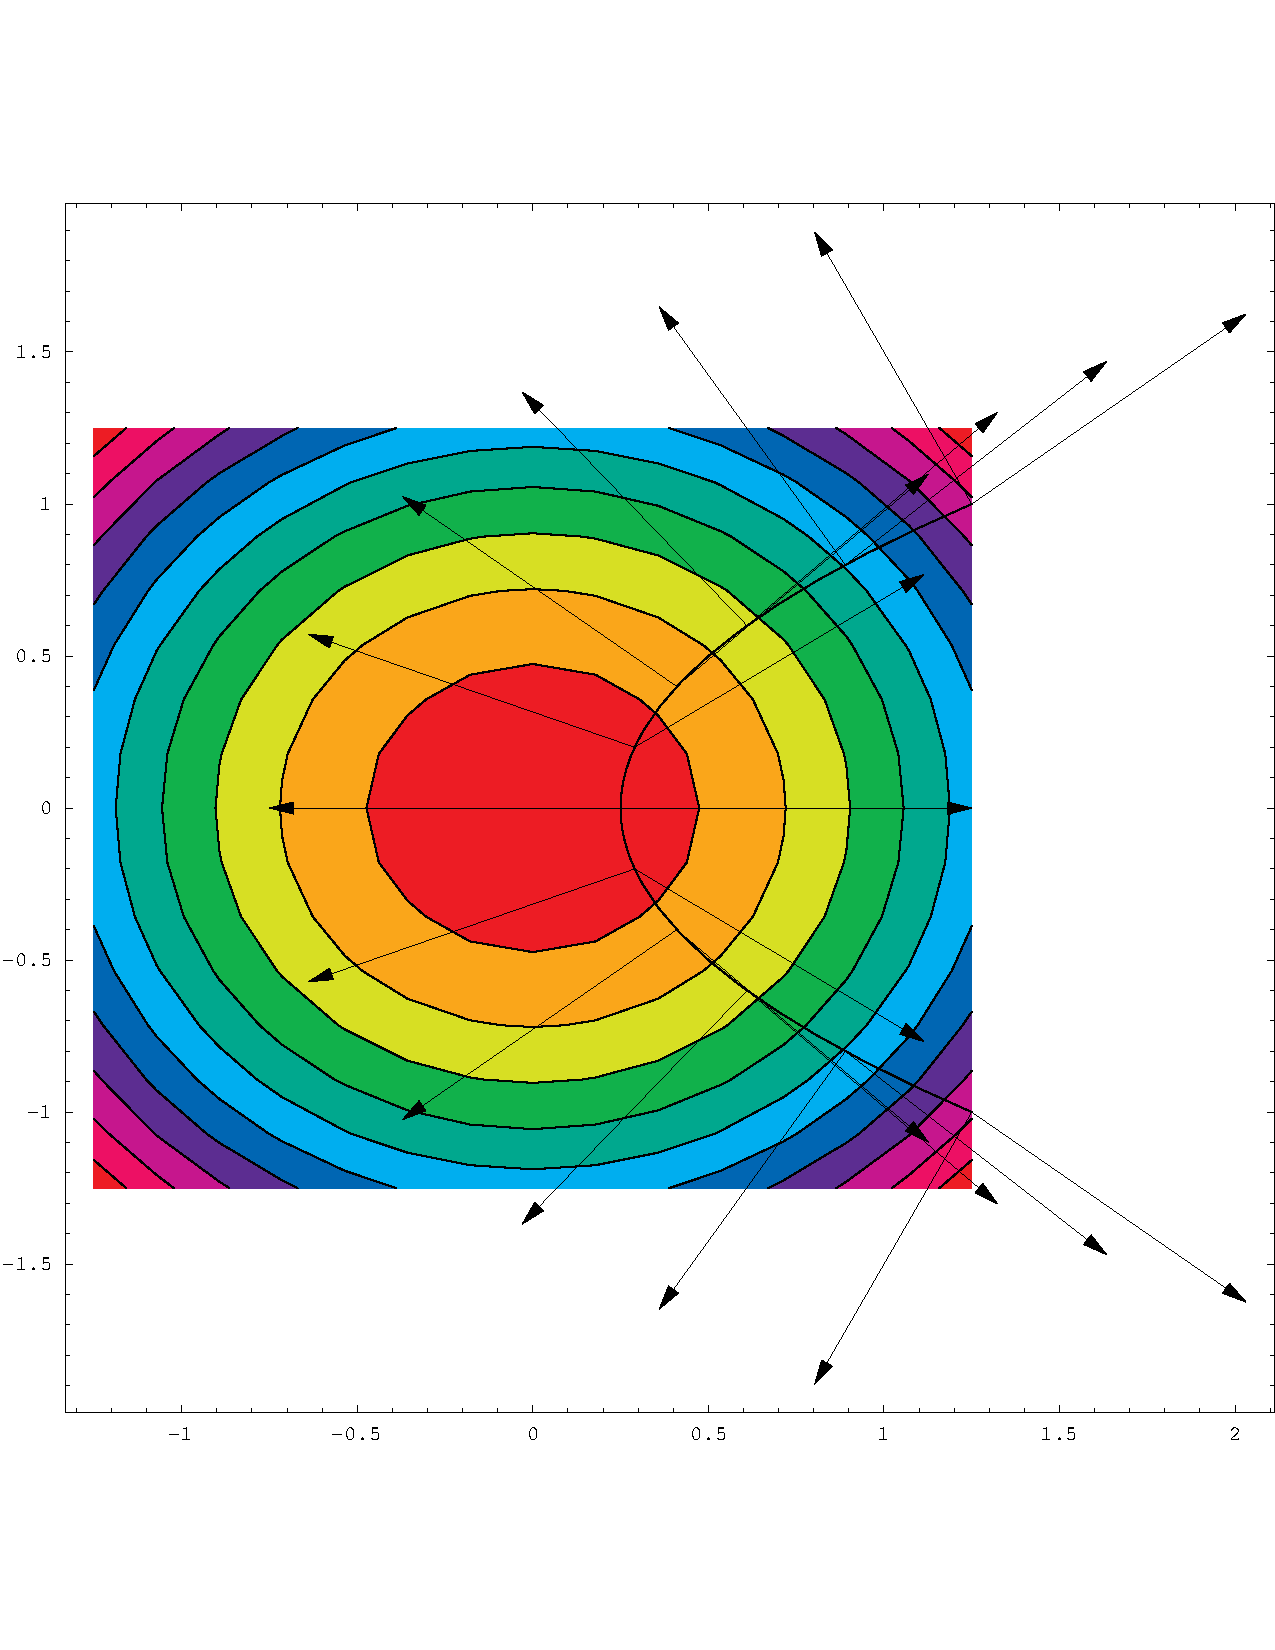
\includegraphics[height=5cm]{figures/ch1/lagrange.pdf}
\caption{Level sets of a convex cost $C$ and a constraint. At the constrained
minimum the gradient of $C$ is balanced by a multiple of the gradient of the
constraint.}
\label{fig:lagrange}
\end{figure}

The last condition is \emph{complementarity}: either the constraint is
active, $A_i(\vx)=b_i$, or its multiplier vanishes. The multiplier is the
force needed to enforce the constraint. In Chapter~\ref{ch:elliptic},
imposed displacements in a Ritz approximation are enforced this way, and the
multipliers are the reaction forces (Section~\ref{ssec:ritz-lagrange}).
Exercises~\ref{exo:kkt1}--\ref{exo:kkt4} work through four cases.

%======================================================================
\section{Galerkin approximation and finite elements}\label{sec:var-fem}
\index{Galerkin method}\index{C\'ea's lemma@C\'ea's lemma}\index{finite element method!one-dimensional}\index{stiffness matrix}%
The weak formulation is exactly what finite element methods discretize:
restrict the problem to a finite-dimensional subspace, solve a linear system,
and control the error with C\'ea's lemma~\cite{Cea1964}
(see also~\cite{Ciarlet2002,BrennerScott2008}).
\begin{center}
\begin{tikzpicture}[node distance=0.55cm]
  \node[box] (a) {Continuous problem in $V$: \ $a(u,v) = L(v)$, infinite-dimensional};
  \node[box, below=of a] (b) {Discrete problem in $V_h \subset V$: \ $a(u_h,v_h) = L(v_h)$};
  \node[box, key, below=of b] (c) {C\'ea's lemma: \ $\norm{u-u_h} \le \frac{M}{\alpha} \inf_{v_h\in V_h} \norm{u-v_h}$};
  \draw[arr] (a) -- (b); \draw[arr] (b) -- (c);
\end{tikzpicture}
\end{center}
Take the one-dimensional problem $-u''=f$ on $(0,1)$, $u(0)=u(1)=0$, with weak
form $\int_0^1u'v'=\int_0^1fv$.
\begin{itemize}
  \item Partition $[0,1]$ into $n$ intervals of size $h=1/n$ and let
  $V_h\subset H^1_0$ be spanned by the piecewise-linear ``hat'' functions
  $\varphi_1,\dots,\varphi_{n-1}$.
  \item Write $u_h=\sum_jc_j\varphi_j$ and require
  $\int u_h'\varphi_i'=\int f\varphi_i$ for each $i$: this is the linear
  system $\mat{K}\mat{c}=\mat{F}$ with the tridiagonal stiffness matrix
  $K_{ij}=\int\varphi_i'\varphi_j'=h^{-1}\operatorname{tridiag}(-1,2,-1)$,
  the matrix of the spring chain.
  \item C\'ea's lemma gives $\norm{u-u_h}_{H^1_0}\le C\inf_{v_h}\norm{u-v_h}_{H^1_0}=O(h)$
  for smooth $u$; nodal values converge faster (Exercise~\ref{exo:conv}).
\end{itemize}
Finite elements for elasticity, with the matrices $\mat{B}$, $\mat{C}$ and
$\mat{B}\T\mat{C}\mat{B}$ of Section~\ref{sec:var-discrete}, are presented in
Chapter~\ref{ch:elliptic}.

%======================================================================
\section{Physical interpretation: energies come first}\label{sec:var-phys}
\index{minimal surface}\index{soap film}%
Many equations of physics and geometry \emph{are} Euler--Lagrange equations of
an energy or action~\cite{GilbargTrudinger2001}: the PDE is a consequence of a
minimization principle, not an artificial reformulation.
\begin{center}
\begin{tikzpicture}[node distance=0.55cm]
  \node[box] (a) {Energy functional $E[u]$ \ (surface area, elastic energy, \dots)};
  \node[box, below=of a] (b) {Critical point: $\delta E(u) = 0$};
  \node[box, goal, below=of b] (c) {Euler--Lagrange equation (PDE), e.g.\ minimal surface equation};
  \draw[arr] (a) -- (b); \draw[arr] (b) -- (c);
\end{tikzpicture}
\end{center}
The area of the graph of $u$ over $\Omega$ is
\[
  A[u]=\int_\Omega\sqrt{1+|\nabla u|^2}\dd x .
\]
A soap film spanning a wire frame (the boundary data) minimizes it. The first
variation $\frac{\dd}{\dd t}A[u+t\varphi]\big|_{t=0}=0$ for all test functions
$\varphi$ gives, after integration by parts (Theorem~\ref{thm:ibp}),
\[
  \dive\!\left(\frac{\nabla u}{\sqrt{1+|\nabla u|^2}}\right)=0,
\]
the minimal surface equation~\cite{Courant1950}. The energy comes first
physically; the PDE follows. The same holds for elasticity, where the stored
energy $\tfrac12\eps:\bbC:\eps$ comes first and the Navier equations follow
(Chapter~\ref{ch:elliptic}).

%======================================================================
\framepart{Summary}
\begin{gbox*}
\begin{itemize}
  \item \textbf{Existence} follows from minimizing a coercive, weakly lower
  semicontinuous energy over a reflexive space
  (Section~\ref{sec:var-direct}); more generally, and without symmetry, from
  the Lax--Milgram theorem (Section~\ref{sec:var-lm}), which covers general
  elliptic operators through G\aa rding's inequality and the Fredholm
  alternative (Section~\ref{sec:var-elliptic}).
  \item \textbf{The weak form} is not an approximation of the strong form
  but a genuine widening of the solution space, made possible by integration
  by parts (Appendix~\ref{app:ibp}).
  \item \textbf{Duality} (Section~\ref{sec:var-dual}) gives every convex
  variational problem a mirror dual problem through the Legendre--Fenchel
  transform; the two meet at the optimum. \textbf{Constraints} enter through
  Lagrange multipliers (Section~\ref{sec:var-lagrange}).
  \item \textbf{The same linear algebra}, $\mat{B}\T\mat{C}\mat{B}\,\vu=\vf$,
  underlies springs, circuits, trusses (Section~\ref{sec:var-discrete}) and
  finite elements (Section~\ref{sec:var-fem}): compatibility, constitutive
  law and equilibrium, with equilibrium the transpose of compatibility.
  \item \textbf{Not every weak form has an energy.} A symmetric form has
  $J(u)=\tfrac12a(u,u)-L(u)$; a non-symmetric one (convection) has none,
  yet Lax--Milgram still applies.
\end{itemize}
\end{gbox*}
The same pattern (energy, weak form, abstract existence theorem, duality,
discretization) appears in linear elasticity, Stokes flow, image denoising by
total variation, and many machine learning objectives written as regularized
energy minimization.

%======================================================================
\framepart{Exercises}\label{sec:var-exo}
Part~I checks results numerically or symbolically: every script was run
(\texttt{numpy}/\texttt{scipy} for numerical checks, \texttt{sympy} for
symbolic ones) and its output is quoted in the comments. Part~II is
paper-and-pencil practice with variational calculus. Part~III treats
constraints and convex conjugates. Solutions are given in small type after
each exercise.

\framesub{Part I: computational verification}

\exercise{Minimizing by gradient descent}\label{exo:gd}
\index{gradient descent}%
For the spring chain ($\mat{K}=\operatorname{tridiag}(-1,2,-1)$,
$\vf=(1,1,1)\T$), minimize $W(\vu)=\tfrac12\vu\T\mat{K}\vu-\vf\T\vu$ by
gradient descent and compare with the direct solution of $\mat{K}\vu=\vf$.
What is the convergence rate?
\begin{solution}
\begin{lstlisting}
import numpy as np
K = np.array([[2,-1,0],[-1,2,-1],[0,-1,2]], dtype=float)
f = np.array([1,1,1], dtype=float)
u, step = np.zeros(3), 0.2
for _ in range(500):
    u -= step * (K @ u - f)              # gradient of W is K u - f
print(np.round(u, 4), np.round(np.linalg.solve(K, f), 4))
# [1.5 2.  1.5] [1.5 2.  1.5]   max difference ~ 1e-15
\end{lstlisting}
The error is multiplied at each step by $\mat{I}-\text{step}\,\mat{K}$, so it
contracts at the rate $\rho=\max_i|1-\text{step}\,\lambda_i(\mat{K})|$
(Figure~\ref{fig:gd}); the eigenvalues are those of Exercise~\ref{exo:lm-constants}.
\end{solution}

\begin{figure}[h]
\centering
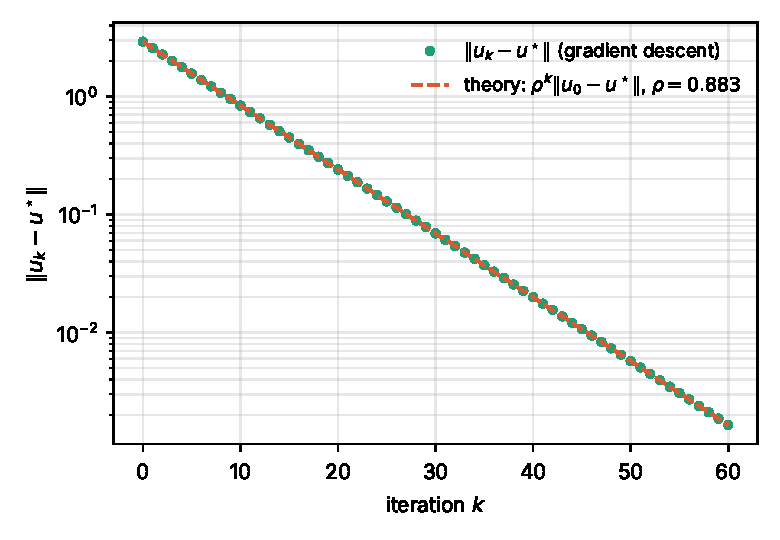
\includegraphics[width=0.55\textwidth]{figures/ch1/ex1_gd_convergence.pdf}
\caption{Exercise~\ref{exo:gd}: the observed convergence of gradient descent
follows the predicted rate $\rho=\max_i|1-\text{step}\,\lambda_i(\mat{K})|$.}
\label{fig:gd}
\end{figure}

\exercise{Integration by parts, checked numerically}\label{exo:ibp-num}
Verify $\int_0^1u'v'\dd x=-\int_0^1u''v\dd x+[u'v]_0^1$ for $u=\sin\pi x$,
$v=x(1-x)$.
\begin{solution}
\begin{lstlisting}
from scipy.integrate import quad
import numpy as np
du  = lambda x: np.pi*np.cos(np.pi*x)
d2u = lambda x: -np.pi**2*np.sin(np.pi*x)
v   = lambda x: x*(1-x);  dv = lambda x: 1-2*x
lhs = quad(lambda x: du(x)*dv(x), 0, 1)[0]
rhs = quad(lambda x: -d2u(x)*v(x), 0, 1)[0] + du(1)*v(1) - du(0)*v(0)
print(lhs, rhs)        # 1.27323954 1.27323954  (= 4/pi)
\end{lstlisting}
\end{solution}

\exercise{Lax--Milgram constants from eigenvalues}\label{exo:lm-constants}
(a) Compute the eigenvalues of the matrix $\mat{K}$ of the spring chain.
(b) Plot the points $(|\vu|^2,\vu\T\mat{K}\vu)$ for many random $\vu$.
(c) Propose two lines bounding the plot. (d) Relate them to the Lax--Milgram
theorem.
\begin{solution}
(a) $\lambda=2-\sqrt2,\ 2,\ 2+\sqrt2$, i.e.\ $0.5858,\ 2,\ 3.4142$.
(b)--(c) Because $\mat{K}$ is symmetric it has an orthonormal eigenbasis
$\ve_1,\ve_2,\ve_3$. Writing $\vu=\sum c_i\ve_i$,
$\vu\T\mat{K}\vu=\sum\lambda_ic_i^2$ and $|\vu|^2=\sum c_i^2$, so
$\alpha|\vu|^2\le\vu\T\mat{K}\vu\le M|\vu|^2$ with $\alpha=\lambda_{\min}$,
$M=\lambda_{\max}$. Both bounds are sharp: equality at $\vu=\ve_1$ and
$\vu=\ve_3$ (Figure~\ref{fig:coercivity}).
(d) The lower line is coercivity, the upper line boundedness: the two
hypotheses of Lax--Milgram, here for the bilinear form $a(\vu,\vv)=\vu\T\mat{K}\vv$.
\begin{lstlisting}
import numpy as np
K = np.array([[2,-1,0],[-1,2,-1],[0,-1,2]], dtype=float)
lam = np.linalg.eigvalsh(K); alpha, M = lam[0], lam[-1]
rng = np.random.default_rng(0)
for _ in range(5):
    u = rng.normal(size=3); a = u @ K @ u
    print(alpha*u@u <= a <= M*u@u)          # True, five times
\end{lstlisting}
\end{solution}

\begin{figure}[h]
\centering
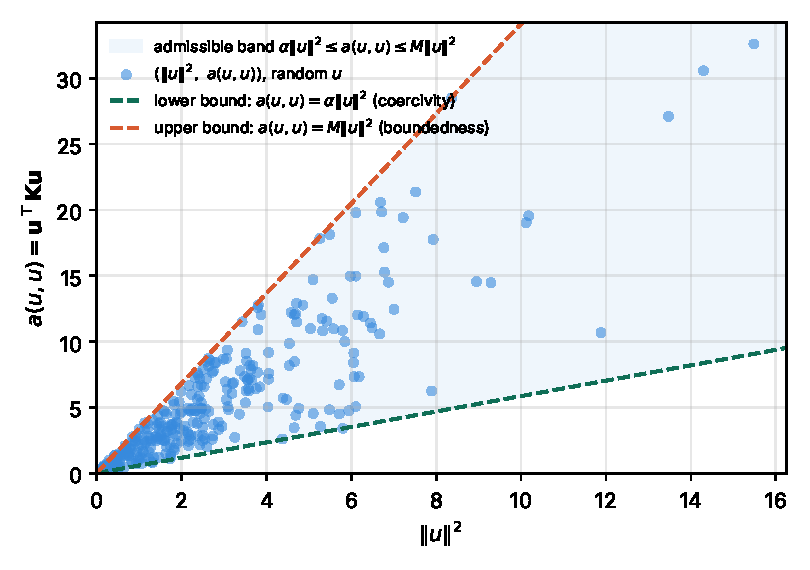
\includegraphics[width=0.6\textwidth]{figures/ch1/ex3_coercivity.pdf}
\caption{Exercise~\ref{exo:lm-constants}: $300$ random vectors $\vu$, plotted
as $(|\vu|^2,\vu\T\mat{K}\vu)$, lie in the band between coercivity
($\alpha|\vu|^2$) and boundedness ($M|\vu|^2$).}
\label{fig:coercivity}
\end{figure}

\exercise{Primal--dual equality for the spring chain}\label{exo:primal-dual}
With $\ve=\mat{B}\vu$ and unit stiffnesses, check that the potential energy
$W(\vu^\ast)$ equals the complementary energy $-\tfrac12|\vect{\sigma}^\ast|^2$
at $\vect{\sigma}^\ast=\mat{B}\vu^\ast$.
\begin{solution}
\begin{lstlisting}
import numpy as np
B = np.array([[1,0,0],[-1,1,0],[0,-1,1],[0,0,-1]], dtype=float)
K, f = B.T @ B, np.ones(3)
u = np.linalg.solve(K, f); s = B @ u
print(0.5*u@K@u - f@u, -0.5*s@s)   # -2.5 -2.5
\end{lstlisting}
Analytically: $W(\vu^\ast)=\tfrac12\vu^{\ast\top}\mat{K}\vu^\ast-\vf\T\vu^\ast=-\tfrac12\vu^{\ast\top}\mat{K}\vu^\ast=-\tfrac12|\mat{B}\vu^\ast|^2$,
the value $W_{\min}$ of Theorem~\ref{thm:min-discrete}.
\end{solution}

\exercise{Convergence rate of the discrete chain}\label{exo:conv}
\index{convergence rate}%
Solve $-u''=\sin\pi x$ on $(0,1)$, $u(0)=u(1)=0$ (exact solution
$\sin(\pi x)/\pi^2$) with the chain matrix for increasing $n$ and measure the
convergence rate.
\begin{solution}
\begin{lstlisting}
import numpy as np
def err(n):
    h = 1.0/(n+1); x = np.linspace(h, 1-h, n)
    K = (2*np.eye(n) - np.eye(n,k=1) - np.eye(n,k=-1))/h**2
    u = np.linalg.solve(K, np.sin(np.pi*x))
    return h, np.max(np.abs(u - np.sin(np.pi*x)/np.pi**2))
for n in [3, 7, 15, 31, 63]: print(*err(n))
# the error is divided by 4 when h is halved: O(h^2)
\end{lstlisting}
The nodal error is $O(h^2)$ (Figure~\ref{fig:conv}), better than the general
$O(h)$ energy-norm bound of C\'ea's lemma, thanks to the smoothness of the
solution.
\end{solution}

\begin{figure}[h]
\centering
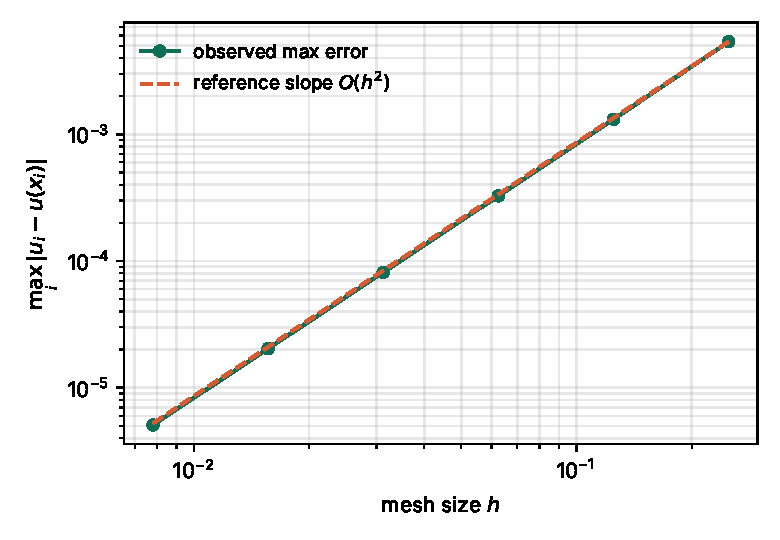
\includegraphics[width=0.55\textwidth]{figures/ch1/ex5_convergence_loglog.pdf}
\caption{Exercise~\ref{exo:conv}: maximal nodal error against $h$; slope $2$.}
\label{fig:conv}
\end{figure}

\exercise{Green's first identity on the unit cube}\label{exo:green-cube}
Verify Green's first identity (Theorem~\ref{thm:green1}) on $\Omega=(0,1)^3$
for $u=xy$, $v=yz$, computing both sides exactly.
\begin{solution}
$\nabla u\cdot\nabla v=(y,x,0)\cdot(0,z,y)=xz$, so the left-hand side is
$\int xz=\tfrac14$. Since $\Delta v=0$, the right-hand side is the boundary
term $\int_{\partial\Omega}u\,\partial_nv$: the faces $z=0$ and $z=1$ give
$\mp\tfrac16$ and cancel, the face $y=1$ gives $\int_0^1\!\!\int_0^1xz\dd x\dd z=\tfrac14$, the others $0$.
\begin{lstlisting}
import sympy as sp
x, y, z = sp.symbols('x y z'); u, v = x*y, y*z
lhs = sp.integrate(sum(sp.diff(u,s)*sp.diff(v,s) for s in (x,y,z)),
                   (x,0,1),(y,0,1),(z,0,1))
faces = [(x,0,-1,(y,z)),(x,1,1,(y,z)),(y,0,-1,(x,z)),
         (y,1,1,(x,z)),(z,0,-1,(x,y)),(z,1,1,(x,y))]
bnd = sum(sp.integrate((u*sg*sp.diff(v,w)).subs(w,val),(a,0,1),(b,0,1))
          for w,val,sg,(a,b) in faces)
print(lhs, bnd)        # 1/4 1/4
\end{lstlisting}
\end{solution}

\exercise{A non-symmetric bilinear form is still solvable}\label{exo:skew}
Add a skew-symmetric convection matrix $b\,\mat{S}$ to the diffusion matrix
$\mat{K}$. Check that $\vu\T(\mat{K}+b\mat{S})\vu=\vu\T\mat{K}\vu$, that
$\mat{K}+b\mat{S}$ is non-symmetric for $b\neq0$, and that the system remains
uniquely solvable.
\begin{solution}
\begin{lstlisting}
import numpy as np
n, h = 5, 1/6
K = (2*np.eye(n) - np.eye(n,k=1) - np.eye(n,k=-1))/h**2
S = (np.eye(n,k=1) - np.eye(n,k=-1))/(2*h)       # S^T = -S
rng = np.random.default_rng(1)
for b in [0.0, 5.0, 50.0]:
    A = K + b*S; u = rng.normal(size=n)
    print(b, np.allclose(A, A.T), np.isclose(u@A@u, u@K@u),
          np.linalg.norm(np.linalg.solve(A, np.ones(n))))
# symmetric only for b = 0; quadratic form unchanged; always solvable
\end{lstlisting}
The skew part vanishes on the diagonal $\vu\T\mat{S}\vu=0$, so coercivity is
unaffected: this is why Lax--Milgram applies without symmetry
(Section~\ref{sec:var-elliptic}).
\end{solution}

\exercise{Reciprocity, componentwise}\label{exo:reciprocity}
Split the degrees of freedom of $\vF=\mat{K}\vu$ into two groups $P$ and $Q$,
\[
  \begin{bmatrix}\vF_P\\ \vF_Q\end{bmatrix}=
  \begin{bmatrix}\mat{K}_{PP}&\mat{K}_{PQ}\\ \mat{K}_{QP}&\mat{K}_{QQ}\end{bmatrix}
  \begin{bmatrix}\vu_P\\ \vu_Q\end{bmatrix}.
\]
Load case 1 loads only $P$, load case 2 only $Q$. Write the reciprocity
identity in blocks and show that it holds for all loads iff
$\mat{K}_{QP}=\mat{K}_{PQ}\T$ (with $\mat{K}_{PP}$, $\mat{K}_{QQ}$ symmetric).
Check it numerically on the spring chain with $P=\{1\}$, $Q=\{3\}$.
\begin{solution}
With $\mat{S}=\mat{K}^{-1}$, case 1 gives $\vu^{(1)}=\mat{S}_{\cdot P}\vF_P^{(1)}$
and case 2 gives $\vu^{(2)}=\mat{S}_{\cdot Q}\vF_Q^{(2)}$. Reciprocity
$\vF^{(1)}\cdot\vu^{(2)}=\vF^{(2)}\cdot\vu^{(1)}$ reads
$\vF_P^{(1)}\cdot\mat{S}_{PQ}\vF_Q^{(2)}=\vF_Q^{(2)}\cdot\mat{S}_{QP}\vF_P^{(1)}$
for all loads, i.e.\ $\mat{S}_{QP}=\mat{S}_{PQ}\T$. Taking also $P=Q$ groups
gives the symmetry of the diagonal blocks, so $\mat{S}$, hence $\mat{K}$, is
symmetric. For the chain, $\mat{S}=\tfrac14\begin{psmallmatrix}3&2&1\\2&4&2\\1&2&3\end{psmallmatrix}$:
a unit load at node~1 moves node~3 by $\tfrac14$, and a unit load at node~3
moves node~1 by $\tfrac14$.
\end{solution}

\framesub{Part II: variational calculus practice}

\paragraph{From energy to strong form, through the weak form.}

\exercise{Natural boundary conditions}\label{exo:neumann}
\index{boundary condition!natural}\index{boundary condition!essential}\index{boundary condition!Neumann}\index{compatibility condition}%
On $\Omega=(0,1)$ consider, over the unconstrained space $V=H^1(0,1)$,
\[
  E[u]=\int_0^1\tfrac12(u')^2\dd x-\int_0^1fu\dd x-g\,u(1).
\]
Derive the weak form, then the strong form and the boundary conditions. What
happens at $x=0$, where $E$ has no boundary term? Is the problem well posed?
\begin{solution}
The first variation is
$\delta E(u)[\varphi]=\int_0^1u'\varphi'-\int_0^1f\varphi-g\varphi(1)=0$ for
all $\varphi\in H^1(0,1)$: this is the weak form. Integrating by parts,
$\int_0^1u'\varphi'=-\int_0^1u''\varphi+u'(1)\varphi(1)-u'(0)\varphi(0)$, so
\[
  \int_0^1(-u''-f)\varphi\dd x+\bigl(u'(1)-g\bigr)\varphi(1)-u'(0)\varphi(0)=0
  \quad\forall\varphi .
\]
Interior test functions give $-u''=f$. Then $\varphi(0)$ and $\varphi(1)$ are
arbitrary (nothing forces them to vanish), so $u'(1)=g$ and $u'(0)=0$. Both
conditions come \emph{for free} from the variational principle: they are
\emph{natural}, as opposed to the \emph{essential} condition $u=0$ of the
model problem, which is built into the space $H^1_0$.

Integrating $-u''=f$ and using both conditions gives the compatibility
condition $g=-\int_0^1f\dd x$: a pure Neumann problem is solvable only if the
data satisfy it (Fredholm alternative), and the solution is unique up to a
constant, on which $E$ does not depend (Figure~\ref{fig:profiles}, left). A
Ritz check with $u=a_0+a_1x+a_2x^2$, $f=1$, $g=-1$:
\begin{lstlisting}
import sympy as sp
x, a0, a1, a2 = sp.symbols('x a0 a1 a2')
u = a0 + a1*x + a2*x**2
E = sp.integrate(sp.diff(u,x)**2/2 - u, (x,0,1)) + u.subs(x,1)
print(sp.diff(E, a0))                                    # 0: a0 free
print(sp.solve([sp.diff(E,a1), sp.diff(E,a2)], [a1,a2])) # a1=0, a2=-1/2
\end{lstlisting}
\end{solution}

\exercise{A reaction term}\label{exo:reaction}
\index{reaction--diffusion}%
Derive the strong form of
$E[u]=\int_\Omega\bigl(\tfrac12|\nabla u|^2+\tfrac12c\,u^2-fu\bigr)\dd x$ over
$H^1_0(\Omega)$, $c>0$ constant.
\begin{solution}
$\delta E(u)[\varphi]=\int_\Omega(\nabla u\cdot\nabla\varphi+cu\varphi-f\varphi)=0$.
Green's first identity on the first term (no boundary term in $H^1_0$) gives
$\int_\Omega(-\Delta u+cu-f)\varphi=0$ for all $\varphi$, hence
$-\Delta u+cu=f$ in $\Omega$, $u=0$ on $\partial\Omega$. Zeroth-order terms in
the energy become zeroth-order terms in the PDE without integration by
parts. In 1D with $c=2$, $f=x$: $u=x/2-\sinh(\sqrt2x)/(2\sinh\sqrt2)$
(Figure~\ref{fig:profiles}, middle).
\end{solution}

\exercise{A nonlinear energy}\label{exo:plaplace}
\index{p-Laplacian@$p$-Laplacian}\index{energy!nonlinear}%
Derive the strong form of $E[u]=\int_0^1\tfrac14(u')^4\dd x-\int_0^1fu\dd x$
over $H^1_0(0,1)$.
\begin{solution}
The density is nonlinear in $u'$; differentiate directly:
$\frac{\dd}{\dd t}\tfrac14(u'+t\varphi')^4\big|_{t=0}=(u')^3\varphi'$. Hence
$\delta E(u)[\varphi]=\int_0^1(u')^3\varphi'-\int_0^1f\varphi=0$, and an
integration by parts gives
\[
  -\bigl((u')^3\bigr)'=f\ \text{in }(0,1),\qquad u(0)=u(1)=0 .
\]
This is the one-dimensional $p$-Laplacian, $-(|u'|^{p-2}u')'=f$ with $p=4$; in
$\R^n$, $-\dive(|\nabla u|^2\nabla u)=f$. The energy penalizes large slopes
more strongly than the quadratic one, which flattens the profile
(Figure~\ref{fig:profiles}, right).
\end{solution}

\begin{figure}[h]
\centering
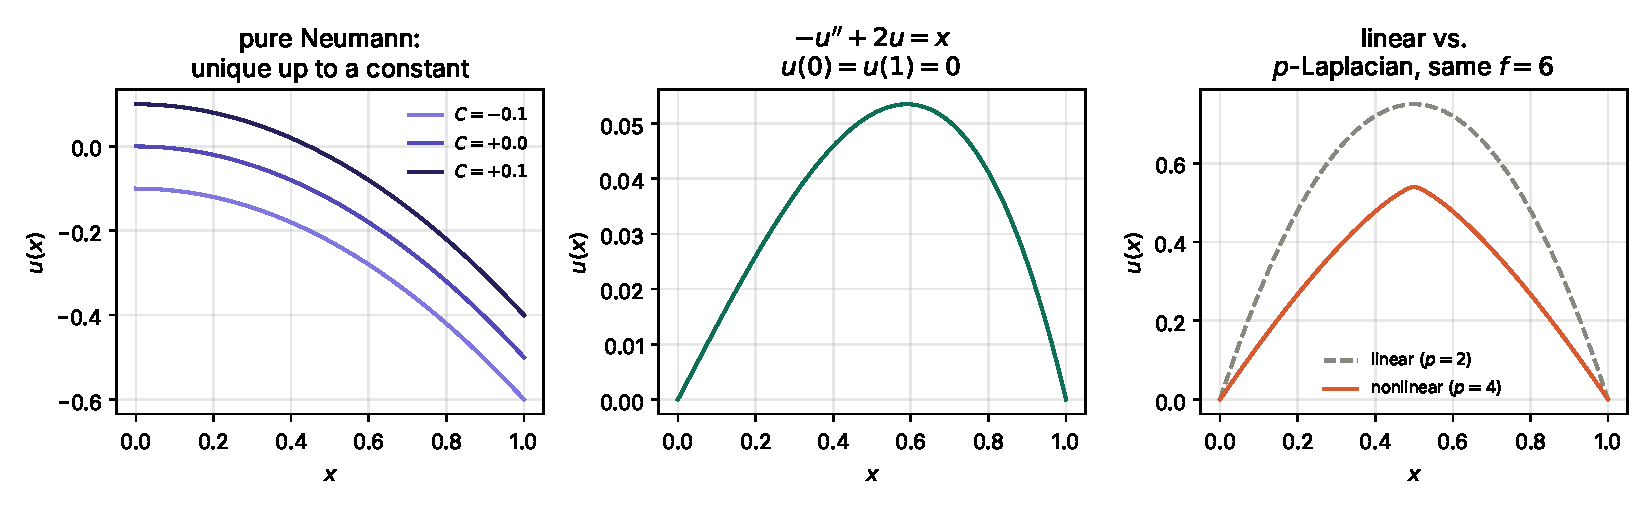
\includegraphics[width=\textwidth]{figures/ch1/ex8_9_10_profiles.pdf}
\caption{Solutions of Exercises~\ref{exo:neumann}--\ref{exo:plaplace}. Left:
the pure Neumann problem is determined up to a constant. Middle: the
reaction--diffusion solution. Right: the nonlinear $p=4$ solution against the
linear $p=2$ solution for the same load $f=6$.}
\label{fig:profiles}
\end{figure}

\paragraph{Guessing the energy from a weak form.}

\exercise{Reconstruct the energy}\label{exo:guess-energy}
\index{energy!from a weak form}%
Find $J$ whose first variation is the weak form: find $u\in H^1(\Omega)$ with
\[
  \int_\Omega\kappa\nabla u\cdot\nabla v\dd x+\int_\Omega\sigma uv\dd x
  =\int_\Omega fv\dd x+\int_{\partial\Omega}gv\dd s\qquad\forall v\in H^1(\Omega),
\]
$\kappa,\sigma>0$ constants.
\begin{solution}
If $a(u,v)=L(v)$ with $a$ \textbf{symmetric} bilinear and $L$ linear, then
$J(u)=\tfrac12a(u,u)-L(u)$ has $\delta J(u)[v]=\tfrac12\bigl(a(u,v)+a(v,u)\bigr)-L(v)=a(u,v)-L(v)$.
Here $a$ is symmetric, so
\[
  J(u)=\tfrac12\int_\Omega\kappa|\nabla u|^2+\tfrac12\int_\Omega\sigma u^2
  -\int_\Omega fu-\int_{\partial\Omega}gu .
\]
\end{solution}

\exercise{When no energy exists}\label{exo:no-energy}
\index{energy!non-existence}%
For the convection--diffusion weak form
$\int_\Omega\nabla u\cdot\nabla v+\int_\Omega(\vb\cdot\nabla u)v=\int_\Omega fv$
on $H^1_0(\Omega)$, $\vb\neq\vzero$ constant, is there an energy $J$ with
$\delta J(u)[v]=a(u,v)-L(v)$?
\begin{solution}
If $J$ existed, its second derivative $a$ would be symmetric (Schwarz's
theorem on mixed derivatives). But for $u,v\in H^1_0$ and constant $\vb$,
integration by parts gives
$\int_\Omega(\vb\cdot\nabla u)v=-\int_\Omega(\vb\cdot\nabla v)u$: the convection
part is \emph{anti}symmetric, so $a(u,v)\neq a(v,u)$ in general. No energy
exists, while Lax--Milgram applies (Section~\ref{sec:var-elliptic}). In 1D
with $b=3$, $u=\sin\pi x$, $v=\sin2\pi x$: $a(u,v)=4$, $a(v,u)=-4$. The skew
part vanishes only on the diagonal $a(u,u)$ (Exercise~\ref{exo:skew}).
\end{solution}

\paragraph{Integration by parts in practice.}

\exercise{Self-adjointness}\label{exo:selfadj}
\index{self-adjointness}%
Let $u,v\in H^2(\Omega)\cap H^1_0(\Omega)$. Use Green's second identity to show
$\int_\Omega u\Delta v=\int_\Omega v\Delta u$.
\begin{solution}
Theorem~\ref{thm:green2} gives
$\int_\Omega(u\Delta v-v\Delta u)=\int_{\partial\Omega}(u\partial_nv-v\partial_nu)$,
and every boundary term contains a vanishing factor $u$ or $v$. This
self-adjointness of the Dirichlet Laplacian is what makes $a(u,v)$ symmetric
and the minimization approach possible.
\end{solution}

\exercise{The Robin problem}\label{exo:robin}
\index{boundary condition!Robin}%
Derive the weak form of $-\Delta u=f$ in $\Omega$, $\partial_nu+\alpha u=g$ on
$\partial\Omega$ ($\alpha>0$), and its energy.
\begin{solution}
Multiply by $v\in H^1(\Omega)$ (Robin, like Neumann, is natural) and use
Green's first identity:
$\int_\Omega\nabla u\cdot\nabla v-\int_{\partial\Omega}\partial_nu\,v=\int_\Omega fv$.
Substituting $\partial_nu=g-\alpha u$:
\[
  \int_\Omega\nabla u\cdot\nabla v+\alpha\int_{\partial\Omega}uv
  =\int_\Omega fv+\int_{\partial\Omega}gv\qquad\forall v\in H^1(\Omega).
\]
The form is symmetric, so
$J(u)=\tfrac12\int_\Omega|\nabla u|^2+\tfrac\alpha2\int_{\partial\Omega}u^2-\int_\Omega fu-\int_{\partial\Omega}gu$.
The Robin condition adds a boundary ``spring'' term, between Dirichlet
($\alpha\to\infty$) and Neumann ($\alpha=0$).
\end{solution}

\exercise{Dirichlet energy from boundary data}\label{exo:dirichlet-energy}
Let $\Delta u=0$ in $\Omega$. Show that
$\int_\Omega|\nabla u|^2=\int_{\partial\Omega}u\,\partial_nu$, and check it on
$(0,1)^3$ for $u=x^2+y^2-2z^2$.
\begin{solution}
Take $v=u$ in Green's first identity; the volume term $\int u\Delta u$
vanishes. The energy of a harmonic field is determined by its boundary data:
this identity is used to compute capacities, and in Chapter~\ref{ch:rg} the
same idea turns boundary measurements into information on a crack. For
$u=x^2+y^2-2z^2$: $\int|\nabla u|^2=\int(4x^2+4y^2+16z^2)=8$; on the boundary, the faces
$x=1$, $y=1$, $z=1$ give $\tfrac43$, $\tfrac43$, $\tfrac{16}3$ and the others $0$: total $8$.
\end{solution}

\framesub{Part III: constraints and convex conjugates}

\exercise{An equality constraint}\label{exo:kkt1}
Minimize $C(\vx)=\tfrac12(x_1^2+x_2^2)$ subject to $x_1-x_2=1$.
\begin{solution}
$\mathcal L=\tfrac12(x_1^2+x_2^2)+\lambda(x_1-x_2-1)$. Stationarity:
$x_1+\lambda=0$, $x_2-\lambda=0$; the constraint gives $-2\lambda=1$. Hence
$\lambda=-\tfrac12$, $\vx=(\tfrac12,-\tfrac12)$, $C=\tfrac14$: the point of the
line closest to the origin.
\end{solution}

\exercise{Two constraints}\label{exo:kkt2}
Minimize $C(\vx)=\tfrac12|\vx|^2$ in $\R^3$ subject to $x_1-x_2=1$ and
$x_2-x_3=2$.
\begin{solution}
Write the constraints $\mat{P}\vx=\vb$ with
$\mat{P}=\begin{psmallmatrix}1&-1&0\\0&1&-1\end{psmallmatrix}$, $\vb=(1,2)$.
Stationarity gives $\vx=-\mat{P}\T\vlambda$, and the constraints
$-\mat{P}\mat{P}\T\vlambda=\vb$ with
$\mat{P}\mat{P}\T=\begin{psmallmatrix}2&-1\\-1&2\end{psmallmatrix}$. Hence
$\vlambda=-(\tfrac43,\tfrac53)$ and $\vx=(\tfrac43,\tfrac13,-\tfrac53)$;
check: $x_1-x_2=1$, $x_2-x_3=2$.
\end{solution}

\exercise{A quadratic form on the circle}\label{exo:kkt3}
\index{eigenvalue problem!as constrained minimization}%
Minimize $C(\vx)=ax_1^2+2bx_1x_2+cx_2^2$ subject to $x_1^2+x_2^2=1$.
\begin{solution}
With $\mat{H}=\begin{psmallmatrix}a&b\\b&c\end{psmallmatrix}$,
$\mathcal L=\vx\T\mat{H}\vx-\lambda(|\vx|^2-1)$ gives $\mat{H}\vx=\lambda\vx$:
the stationary points are the unit eigenvectors, and $C=\lambda$ there. The
minimum is the smallest eigenvalue,
$\tfrac{a+c}2-\sqrt{\bigl(\tfrac{a-c}2\bigr)^2+b^2}$. Constrained minimization
of a quadratic form is an eigenvalue problem: this is the root of the
Rayleigh quotient, of~\eqref{eq:rayleigh}, and of the buckling problems later
in the course.
\end{solution}

\exercise{The saddle-point system}\label{exo:kkt4}
\index{saddle point!system}%
Minimize $C(\vx)=\tfrac12\vx\T\mat{H}\vx-\vx\T\vf$, $\mat{H}$ symmetric
positive definite, subject to $\mat{P}\vx=\vb$ ($\mat{P}$ of full row rank).
\begin{solution}
$\mathcal L=C(\vx)+\vlambda\cdot(\mat{P}\vx-\vb)$, and stationarity in
$(\vx,\vlambda)$ gives
\[
  \begin{bmatrix}\mat{H}&\mat{P}\T\\ \mat{P}&\mat{0}\end{bmatrix}
  \begin{bmatrix}\vx\\ \vlambda\end{bmatrix}=
  \begin{bmatrix}\vf\\ \vb\end{bmatrix},
  \qquad
  \vlambda=(\mat{P}\mat{H}^{-1}\mat{P}\T)^{-1}(\mat{P}\mat{H}^{-1}\vf-\vb),\quad
  \vx=\mat{H}^{-1}(\vf-\mat{P}\T\vlambda).
\]
The matrix is symmetric but indefinite: $(\vx,\vlambda)$ is a saddle point,
a minimum in $\vx$ and a maximum in $\vlambda$. This is the system used for
imposed displacements in Chapter~\ref{ch:elliptic}.
\end{solution}

\exercise{Legendre--Fenchel transforms}\label{exo:lf}
(a) Give a geometric interpretation of $F^\ast$ in $\R^2$ and prove the
Fenchel--Young inequality. (b) Compute $F^\ast$ for $F(x)=x^2$, $F(x)=x^4$,
$F(x)=e^x$, and the indicator $F(x)=0$ for $x\le0$, $+\infty$ for $x>0$.
\begin{solution}
(a) $F^\ast(p)$ is the largest gap between the line $px$ and the graph of
$F$; the line $px-F^\ast(p)$ is the supporting line of slope $p$
(Figure~\ref{fig:legendre}). By definition $F^\ast(p)\ge px-F(x)$ for every
$x$, which is Fenchel--Young; equality holds where the supremum is attained,
$p=F'(x)$.
(b) $x^2$: the maximum of $px-x^2$ is at $x=p/2$, $F^\ast(p)=p^2/4$.
$x^4$: $p=4x^3$, $F^\ast(p)=3(p/4)^{4/3}$.
$e^x$: $F^\ast(p)=p\ln p-p$ for $p>0$, $0$ for $p=0$, $+\infty$ for $p<0$.
Indicator of $\{x\le0\}$: $F^\ast(p)=\sup_{x\le0}px$, which is $0$ for $p\ge0$
and $+\infty$ for $p<0$, the indicator of $\{p\ge0\}$. This last pair is the
convex-analysis form of the complementarity conditions of
Section~\ref{sec:var-lagrange}, and reappears in plasticity.
\end{solution}

%======================================================================
\begin{chapterbib}{99}
\bibitem{AdamsFournier2003} R.~A.~Adams, J.~J.~F.~Fournier, \emph{Sobolev Spaces}, 2nd ed., Academic Press, 2003.
\bibitem{AllenCahn1979} S.~M.~Allen, J.~W.~Cahn, A microscopic theory for antiphase boundary motion and its application to antiphase domain coarsening, \emph{Acta Metall.} 27 (1979) 1085--1095.
\bibitem{BrennerScott2008} S.~C.~Brenner, L.~R.~Scott, \emph{The Mathematical Theory of Finite Element Methods}, 3rd ed., Springer, 2008.
\bibitem{Brezis2011} H.~Brezis, \emph{Functional Analysis, Sobolev Spaces and Partial Differential Equations}, Springer, 2011.
\bibitem{Cea1964} J.~C\'ea, Approximation variationnelle des probl\`emes aux limites, \emph{Ann. Inst. Fourier} 14 (1964) 345--444.
\bibitem{Ciarlet2002} P.~G.~Ciarlet, \emph{The Finite Element Method for Elliptic Problems}, SIAM Classics in Applied Mathematics 40, 2002.
\bibitem{Courant1950} R.~Courant, \emph{Dirichlet's Principle, Conformal Mapping, and Minimal Surfaces}, Interscience, 1950.
\bibitem{Dacorogna2008} B.~Dacorogna, \emph{Direct Methods in the Calculus of Variations}, 2nd ed., Springer, 2008.
\bibitem{EkelandTemam1999} I.~Ekeland, R.~Temam, \emph{Convex Analysis and Variational Problems}, SIAM Classics in Applied Mathematics 28, 1999.
\bibitem{Evans2010} L.~C.~Evans, \emph{Partial Differential Equations}, 2nd ed., AMS, 2010.
\bibitem{Garding1953} L.~G\aa rding, Dirichlet's problem for linear elliptic partial differential equations, \emph{Math. Scand.} 1 (1953) 55--72.
\bibitem{GilbargTrudinger2001} D.~Gilbarg, N.~S.~Trudinger, \emph{Elliptic Partial Differential Equations of Second Order}, Springer Classics in Mathematics, 2001.
\bibitem{LaxMilgram1954} P.~D.~Lax, A.~N.~Milgram, Parabolic equations, in \emph{Contributions to the Theory of Partial Differential Equations}, Ann. Math. Studies 33, Princeton, 1954, 167--190.
\bibitem{Rockafellar1970} R.~T.~Rockafellar, \emph{Convex Analysis}, Princeton University Press, 1970.
\bibitem{Strang1986} G.~Strang, \emph{Introduction to Applied Mathematics}, Wellesley-Cambridge Press, 1986.
\end{chapterbib}
